\subsection{Detec��o de Bordas \label{deteccao_de_bordas}}

Detec��o de Bordas � uma t�cnica para localizar os pontos e linhas que
dividem regi�es distintas de uma determinada imagem. A detec��o das
bordas pode ser feita atrav�s do uso de diversos operadores.
Computacionalmente, define-se uma borda como sendo uma regi�o que possui
um gradiente de alta magnitude, por este fato, o operador de Sobel � uma
interessante forma de se realizar a detec��o de bordas, visto que este
operador � baseado no c�lculo do gradiente e sua magnitude.

Segundo \cite{MADRUGA_2005} e \cite{FELGUEIRAS_2006}, o c�lculo do
gradiente � dado por:

\begin{large}
\begin{center}
    $\nabla f =  \begin{bmatrix} Gx \\ Gy \end{bmatrix} =
    \begin{bmatrix} \frac{\partial f}{\partial x} \\ \frac{\partial f}{\partial y} \end{bmatrix}$
\end{center}
\end{large}

E sua magnitude � dada por:
\begin{large}
\begin{center}
    $ mag(\nabla f) = [ G_x^2 + G_y^2 ]^\frac{1}{2} $
\end{center}
\end{large}

Onde:

\begin{large}
\begin{center}
    $G_x =  \begin{bmatrix} -1 & 0 & 1 \\
                                    -2 & 0 & 1 \\
                                    -1 & 0 & 1
                \end{bmatrix}
    $ e $
              \begin{bmatrix} 1 & 2 & 1 \\
                                    0 & 0 & 0 \\
                                    -1 & -2 & -1
                \end{bmatrix}
    $
\end{center}
\end{large}

s�o operadores que aplicam o processo de convolu��o na imagem como visto no t�pico anterior.

Atrav�s destes c�lculos � poss�vel obter, al�m da magnitude, a
dire��o do gradiente.

\begin{figure}[h|top]
 \centering
 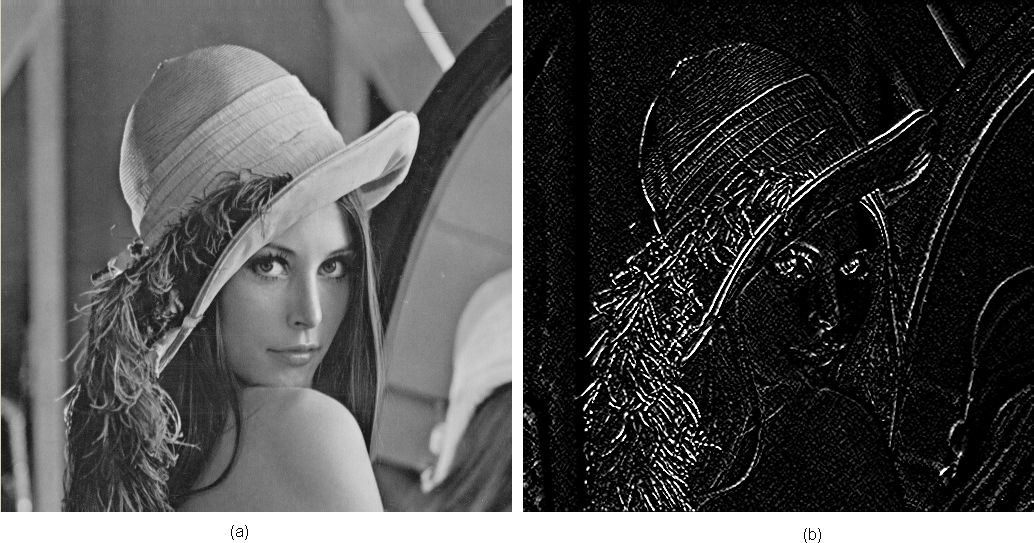
\includegraphics[width=0.7\linewidth]{imagens/filtragem_sobel.png}
 \caption{a) Imagem Original; b) Imagem ap�s sofrer filtragem com operador de Sobel.}
 \label{img_sobel}
\end{figure}


Observa-se na Figura \ref{img_sobel}, que ao realizar uma filtragem
utilizando o operador de Sobel, a imagem tem suas bordas em maior
destaque do que na imagem original (Figura \ref{img_sobel} - a )
Apesar deste operador realizar uma boa detec��o de bordas, ele
tamb�m aumenta o n�vel dos ru�dos da imagem. Isto se deve ao fato de
que ao passar pelos processos de convolu��o e c�lculo de magnitude
do gradiente, os ru�dos, assim como as bordas, retornam um valor de
magnitude elevada, sendo necess�rio aplicar outros processos de
filtragem para a redu��o dos mesmos.

Neste trabalho ser�o utilizadas algumas t�cnicas de Filtragem
Espacial para fazer o realce das bordas do ritmo visual,
possibilitando dar um destaque maior para as bordas que possam
possivelmente caracterizar uma transi��o.

Uma melhor abordagem sobre estes m�todos pode ser encontrada em
\cite{MADRUGA_2005} , \cite{FELGUEIRAS_2006} ,
\cite{STIVANELLO_2005} , \cite{SANTOS_2005} e \cite{BOTELHO_2007}.
